\documentclass[preprint,12pt]{elsarticle}
\usepackage{amsmath,amssymb}
\usepackage{graphicx}
\usepackage{booktabs}
\usepackage{multirow}
\usepackage{xcolor}
\usepackage{xurl}
\usepackage{lineno}
\usepackage{tikz}
\usetikzlibrary{arrows.meta,positioning}
\usepackage[hidelinks]{hyperref}
% Draft markers: red text must be checked or filled before submission.
\newcommand{\todo}[1]{\textcolor{red}{[TODO: #1]}}
\journal{Optical Switching and Networking}

\begin{document}
\begin{frontmatter}

\title{Does Knowing the Traffic Pattern Help? Periodic-Flow Detection, Spectrum Reservation and Grouped Push-Pull Defragmentation in Elastic Optical Networks}

\author[qom]{Mohammad Mahdi Malayeri}
\ead{malayerimahdi@gmail.com}
\author[qom]{Mohsen Nickray\corref{cor1}}
\ead{\todo{email}}
\cortext[cor1]{Corresponding author. \todo{Confirm the corresponding author with Dr Nickray.}}
\affiliation[qom]{organization={Department of Computer Engineering and Information Technology, University of Qom},
            city={Qom},
            country={Iran}}

\begin{abstract}
Spectrum fragmentation causes requests in elastic optical networks (EONs) to be blocked even when enough total capacity is free. Scheduled services such as IPTV repeat between the same node pairs, and this paper tests whether that regularity can be used to allocate spectrum better. Periodic flows are detected from the request stream with a training-free rule and used in four ways: advance spectrum reservation, a separate spectrum zone, holding spectrum between repeats, and holding with a budget on idle spectrum. All schemes use non-disruptive Push-Pull defragmentation, with shifts grouped into parallel rounds by a greedy maximal-independent-set algorithm. Simulations on NSFNET and Germany50 with paired statistical tests show that defragmentation provides the reliable gains: Push-Pull lowers bandwidth blocking by 24--92\% compared with First-Fit, and route grouping makes it 2.5--3.7 times faster. Periodic flows are detected with a precision of 1.00 and a recall of 0.86--0.99, yet no use of them lowers total blocking. Holding spectrum protects periodic flows by up to 41\% and a separate zone cuts defragmentation shifts by up to 61\%, but both raise the blocking of other traffic. The trade-off can be tuned: reserving spectrum about one tenth of a period ahead lowers the blocking of periodic flows by 29--49\% without a significant change in total blocking, on both topologies and for periodic shares of 10--50\%. Under timing jitter, a detection tolerance of three times the jitter keeps the recall above 0.8. Pattern awareness thus does not create capacity; it decides which traffic receives it.
\end{abstract}

\begin{highlights}
\item Periodic flows are detected from the request stream without training.
\item Push-Pull cuts blocking 24--92\%; route grouping makes it 2.5--3.7$\times$ faster.
\item Knowing traffic patterns redistributes spectrum but does not lower total blocking.
\item Short-lead reservation protects periodic flows 29--49\% at no total cost.
\item Results hold on NSFNET and Germany50; simulator and data are open.
\end{highlights}

\begin{keyword}
Elastic optical networks \sep Spectrum fragmentation \sep Push-Pull defragmentation \sep Traffic pattern recognition \sep Advance reservation \sep Independent sets
\end{keyword}

\end{frontmatter}

\linenumbers

% ===============================================================
\section{Introduction}
% ===============================================================
Elastic optical networks (EONs) divide the optical spectrum into fine-grained frequency slots (FSs) and give each connection only as many contiguous slots as it needs \cite{jinno2009,gerstel2012}. A lightpath must use the same contiguous block of slots on every link of its route, which is known as the spectrum continuity and contiguity constraint \cite{chatterjee2015,talebi2014}. As connections with different bandwidths and holding times are set up and released, the free spectrum breaks into small gaps that are not aligned across links. A new request can then be blocked even though enough total capacity is free. This spectrum fragmentation is one of the main obstacles to running dynamic EONs efficiently.

Two families of methods address fragmentation. Fragmentation-aware routing and spectrum assignment (RSA) tries to avoid creating unusable gaps \cite{shen2015,abkenar2017,athari2019}, and defragmentation re-arranges active connections to consolidate free spectrum \cite{patel2011,wang2013,zhang2013,cugini2013}. Both act on the current state of the spectrum and treat future requests as unknown. Real traffic, however, is not purely random. Scheduled services such as IPTV, video on demand and periodic backups repeat between the same node pairs with nearly constant intervals and bandwidths. A natural idea is to recognize such patterns and act before the requests arrive. This idea was explored in the MSc thesis on which this paper builds \cite{malayeri2022}, where a pattern finder on the request stream was combined with Push-Pull defragmentation in an OPNET model of NSFNET. The gains reported there were small, and it was not clear whether this was a property of the idea or of the experiment.

This paper revisits the question with a controlled experiment. We build an open discrete-event simulator in which the share of periodic traffic is an explicit parameter, so that pattern-aware schemes can be compared with pattern-blind ones under identical traffic. We then ask three questions:
\begin{enumerate}
\item How much of the benefit comes from defragmentation itself, and how much from knowing the pattern?
\item Can periodic flows be detected reliably from the request stream, including when their arrival times are noisy?
\item Which way of using the detected patterns gives the best trade-off between protecting periodic flows and serving the rest of the traffic?
\end{enumerate}

The main contributions are:
\begin{itemize}
\item A periodic-flow detector that runs on the request stream with constant work per request, and four ways to use its output: advance reservation, a separate spectrum zone, holding spectrum between repeats, and holding with a budget on idle spectrum.
\item A grouped Push-Pull defragmentation in which routes that share no link are shifted in parallel, using a greedy maximal-independent-set partition of the moved routes \cite{shakya2013}.
\item An evaluation on two topologies (NSFNET and the 50-node Germany50 network from SNDlib \cite{orlowski2010}), with 10 independent runs per point, 95\% confidence intervals and paired significance tests, which shows clearly what pattern awareness can and cannot achieve.
\item A sensitivity study of the reservation lead time, the hold budget, the share of periodic traffic and the detection tolerance under timing jitter, which identifies advance reservation with a moderate lead as the most efficient way to protect periodic flows.
\item An open-source simulator with all experiment scripts and raw results, so that every number in this paper can be reproduced.\footnote{\url{https://github.com/malayerimahdi/EON-Pattern-Aware-Spectrum-Management}}
\end{itemize}

The rest of the paper is organized as follows. Section~\ref{sec:related} reviews related work. Section~\ref{sec:model} defines the network and traffic model. Section~\ref{sec:method} describes the methods. Section~\ref{sec:setup} gives the simulation setup, Section~\ref{sec:results} the results, and Section~\ref{sec:discussion} discusses them. Section~\ref{sec:conclusion} concludes the paper.

% ===============================================================
\section{Related Work}\label{sec:related}
% ===============================================================
\subsection{Routing, spectrum assignment and fragmentation}
Surveys of RSA and spectrum management in EONs are given in \cite{chatterjee2015,abkenar2017,talebi2014}. Most dynamic RSA schemes compute $k$ shortest paths \cite{yen1971} and choose a spectrum position with First-Fit or a variant of it. Fragmentation-aware RSA chooses positions that limit small gaps, for example by measuring how a candidate allocation changes the fragmentation of the affected links \cite{shen2015}, or by combining such measures with learning in space-division multiplexing EONs \cite{athari2019}. These schemes reduce the rate at which fragmentation builds up, but cannot remove it.

\subsection{Defragmentation}
Defragmentation re-arranges active lightpaths to consolidate free spectrum \cite{patel2011}. Because re-tuning a lightpath can interrupt its traffic, later work proposed make-before-break and non-disruptive variants \cite{wang2013,zhang2013}. Push-Pull defragmentation shifts a lightpath to adjacent free slots by slowly re-tuning the transmitter and receiver, so that no traffic is lost \cite{cugini2013}. A lightpath cannot jump over another one, which limits how far it can move, but the operation is hitless. Since lightpaths on routes that share no link do not interact, independent sets of routes can be defragmented in parallel \cite{shakya2013}. We use this idea to group the shifts of each Push-Pull pass into parallel rounds.

\subsection{Learning and traffic awareness}
Advance reservation, where requests are known before they start, allows better planning of spectrum use \cite{lu2013ar}. Spectrum allocation adapted to estimated traffic fluctuations was studied in \cite{chino2016}. Machine learning has been applied to bandwidth allocation with quality-of-service constraints \cite{panayiotou2019}, to RSA with learned quality-of-transmission estimates \cite{salani2019}, and to routing, modulation and spectrum assignment with deep reinforcement learning \cite{chen2019}. Learning has also been applied to defragmentation itself. Deep reinforcement learning has been used to select which connections to re-allocate and when \cite{etezadi2022,etezadi2023}, a classifier has been used to trigger defragmentation when the predicted blocking exceeds a threshold \cite{davalos2023}, and cognitive control loops have been proposed to detect and repair degraded network states \cite{trindade2021}. Open toolkits such as the Optical RL-Gym have made such studies easier to reproduce \cite{natalino2020}.

These works learn \emph{when} or \emph{how} to defragment, or how to route a request that has already arrived. We instead learn \emph{which demands recur}, from the request stream itself and without a training phase, and we measure under identical traffic how each way of using this knowledge changes blocking and defragmentation cost. To our knowledge, no previous study has compared reservation, zoning and holding for detected periodic flows side by side, or separated the effect of pattern knowledge from that of the defragmentation it is combined with.

% ===============================================================
\section{Network and Traffic Model}\label{sec:model}
% ===============================================================
The network is an undirected graph $G=(V,E)$ in which each link carries $S$ frequency slots. A request is a tuple $r=(t_r, s_r, d_r, b_r, h_r)$ of arrival time, source, destination, number of FSs and holding time. It is served on one of the $k$ shortest paths between $s_r$ and $d_r$ if $b_r+g$ contiguous FSs, where $g$ is the guard band, are free at the same position on every link of the path. Otherwise it is blocked. We use a single modulation format, so that the results reflect spectrum management only and not distance-adaptive transmission.

The traffic follows the generator of \cite{malayeri2022}: requests arrive as a Poisson process between uniformly chosen node pairs, $b_r$ is uniform in 5--20 FSs, and holding times are exponential with mean $\bar{h}$. On top of this random traffic, $F$ periodic flows each repeat a fixed tuple $(s,d,b)$ with a constant period. A share $\phi$ of the offered load $A$ (in Erlang) comes from the periodic flows. Random requests therefore arrive at rate $(1-\phi)A/\bar{h}$, and each periodic flow has period
\begin{equation}
T = \frac{F\,\bar{h}}{\phi A}.
\end{equation}
Real scheduled services do not start exactly on time. In the robustness experiments we therefore add independent Gaussian noise with standard deviation $\sigma$ to the arrival time of every periodic request, clipped to $\pm T/4$, while the nominal schedule stays periodic.

% ===============================================================
\section{Methods}\label{sec:method}
% ===============================================================
Fig.~\ref{fig:pipeline} shows how the components fit together. Every request updates the detector. Requests are placed with First-Fit (Last-Fit in the periodic zone, when used). When a request is blocked, grouped Push-Pull is run and the request is tried again. Detected periodic flows trigger one of the pattern-based actions.

\begin{figure}[t]
\centering
\resizebox{\textwidth}{!}{%
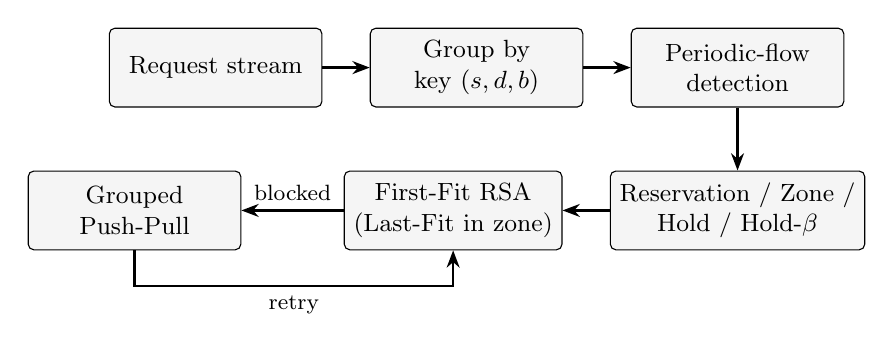
\begin{tikzpicture}[
  box/.style={draw, rounded corners=2pt, align=center, font=\small, minimum width=2.7cm, minimum height=1.0cm, fill=gray!8},
  arr/.style={-{Stealth[length=2.2mm]}, thick}]
\node[box] (a) {Request stream};
\node[box, right=0.6cm of a] (b) {Group by\\key $(s,d,b)$};
\node[box, right=0.6cm of b] (c) {Periodic-flow\\detection};
\node[box, below=0.8cm of c] (d) {Reservation / Zone /\\Hold / Hold-$\beta$};
\node[box, left=0.6cm of d] (e) {First-Fit RSA\\(Last-Fit in zone)};
\node[box, left=1.3cm of e] (f) {Grouped\\Push-Pull};
\draw[arr] (a)--(b); \draw[arr] (b)--(c); \draw[arr] (c)--(d); \draw[arr] (d)--(e);
\draw[arr] (e)--node[above, font=\footnotesize]{blocked} (f);
\draw[arr] (f.south) |- ++(0,-0.45) -| node[pos=0.25, below, font=\footnotesize]{retry} (e.south);
\end{tikzpicture}}
\caption{Components of the pattern-aware scheme.}
\label{fig:pipeline}
\end{figure}

\subsection{Grouped Push-Pull defragmentation}
When a request is blocked, Push-Pull \cite{cugini2013} visits the active lightpaths in order of their lowest slot and shifts each one to the lowest position it can reach through contiguous free slots on all links of its route. A shift never jumps over another lightpath, so it does not disrupt traffic. After the pass, the blocked request is tried again.

Shifts on routes that share no link can be performed at the same time. We build a conflict graph whose vertices are the routes of the lightpaths moved in the pass, with an edge between two routes that share a link. We then repeatedly remove a maximal independent set from this graph, taking shorter routes first, as in \cite{shakya2013}. Each set is one parallel round. Because a single re-tuning step takes the same time for all lightpaths, the number of rounds, rather than the number of shifts, sets the duration of defragmentation. The order of shifts within a pass is kept, so grouping does not change the final spectrum state; it only changes how long it takes to reach it.

\subsection{Periodic-flow detection}
Requests are grouped by their key $(s,d,b)$. For each key we keep the last four arrival times $t_1<t_2<t_3<t_4$. Let $T$ be the mean of the three intervals. The key is marked periodic with period $T$ if
\begin{equation}
\left| (t_{i+1}-t_i) - T \right| \le \varepsilon,\qquad i=1,2,3,
\end{equation}
where $\varepsilon$ is the detection tolerance ($\varepsilon=0.1$ unless stated). A key loses its mark as soon as an interval breaks the rule. The next arrival of a periodic key is expected at $t_4+T$. This rule is a stream version of the pattern finder of \cite{malayeri2022}: it needs no training phase and costs $O(1)$ work and memory per key.

\subsection{Four uses of detected patterns}
\paragraph{Reservation} A lead time $\delta$ before the next expected arrival of a periodic key, a block of $b$ FSs is reserved on one of its $k$ paths, with Push-Pull if needed. The arriving request takes the reserved block. If it does not arrive within $\varepsilon+\delta$ of the expected time, the block is released. The reserved block is idle for about $\delta$, so the lead time sets the price of the reservation.

\paragraph{Zone} Detected periodic flows are placed with Last-Fit, at the top of the band, while all other traffic uses First-Fit from the bottom. Push-Pull pushes periodic connections up and the others down. The goal is to keep the two classes from fragmenting each other.

\paragraph{Hold} When a connection of a periodic key ends and its next repeat is still expected, its block is kept for that repeat instead of being released. The next request of the key takes the held block.

\paragraph{Hold with a budget} A held block is idle for the whole gap between two repeats. To control this cost, a block is held only if, on every link of its route, the slots already idle in held or reserved blocks plus the new block stay within a share $\beta$ of the $S$ slots. Otherwise it is released as usual. $\beta=1$ gives unrestricted Hold and $\beta\to 0$ gives FF+PP.

\subsection{Per-pair demand prediction}
The thesis \cite{malayeri2022} also proposed to predict the demand of each node pair. To test whether this is possible, time is divided into windows. For each pair, a decision tree (depth 5) predicts from the demands of the previous three windows whether the next window's demand will exceed a threshold, defined as the mean demand per pair and window. The first 70\% of windows are used for training and the rest for testing.

\subsection{Complexity}
Detection costs $O(1)$ per request. A First-Fit search on a path of $\ell$ links costs $O(\ell S)$. One Push-Pull pass over $n$ active lightpaths costs $O(n\,\ell S)$ in the worst case, and the greedy grouping of $m$ moved routes costs $O(m^2\ell)$, which is small next to the shift operations it schedules. Checking the hold budget costs $O(\ell)$ if a counter of idle slots is kept per link. None of the pattern-based actions changes the order of these costs.

% ===============================================================
\section{Simulation Setup}\label{sec:setup}
% ===============================================================
We use a Python discrete-event simulator written for this study. It is released with all experiment scripts and raw results. After every run, a consistency check verifies that the spectrum map matches the set of active connections and that no two lightpaths overlap.

\paragraph{Topologies} The main topology is the 14-node, 21-link NSFNET used in \cite{malayeri2022}, with link lengths of 300--2800\,km. To test whether the findings generalize, we repeat the main experiments on Germany50 from SNDlib \cite{orlowski2010}, a 50-node, 88-link national network. Its link lengths (26--252\,km) are computed as great-circle distances between the node coordinates. Since we use a single modulation format, lengths affect only the choice of the $k$ shortest paths. Germany50 has many more node pairs and longer paths in hops, so the same blocking range is reached at a similar offered load as on NSFNET.

\paragraph{Parameters} Table~\ref{tab:params} lists the parameters. Each run simulates 20{,}000 requests after a warm-up of 2{,}000 requests, and each point is the mean of 10 independent seeds. At 100 Erlang and $\phi=0.3$ the period of each periodic flow is $T\approx13.3$.

\begin{table}[t]
\centering
\caption{Simulation parameters.}
\label{tab:params}
\small
\begin{tabular}{@{}ll@{}}
\toprule
Parameter & Value \\
\midrule
Topologies & NSFNET (14 nodes, 21 links) \\
 & Germany50 (50 nodes, 88 links) \\
FSs per link $S$ / guard band $g$ & 320 / 1 FS \\
Routing / assignment & $k=3$ shortest paths \cite{yen1971} / First-Fit \\
Demand $b_r$ & uniform, 5--20 FSs \\
Mean holding time $\bar{h}$ & 20 \\
Periodic flows $F$ / share $\phi$ & 20 / 0.3 (0.1--0.5 in Section~\ref{sec:phi}) \\
Offered load $A$ & 50--120 Erlang (NSFNET) \\
 & 70--150 Erlang (Germany50) \\
Detection tolerance $\varepsilon$ & 0.1 (0.3 in Section~\ref{sec:jitter}) \\
Reservation lead $\delta$ & 0.2 (0.2--5 in Section~\ref{sec:tradeoff}) \\
Hold budget $\beta$ & 1 (0.02--0.2 in Section~\ref{sec:tradeoff}) \\
Requests per run & 20{,}000 after 2{,}000 warm-up \\
Runs per point & 10 seeds \\
\bottomrule
\end{tabular}
\end{table}

\paragraph{Schemes} We compare First-Fit without defragmentation (FF), FF with grouped Push-Pull (FF+PP), and FF+PP with each use of detected patterns: Reservation, Zone, Hold, Zone+Hold and Hold with a budget $\beta$.

\paragraph{Metrics} We report the bandwidth blocking probability (BBP), i.e., the share of requested FSs that are blocked, and the request blocking probability (BP) of periodic and of random requests separately. For defragmentation we report the number of Push-Pull shifts and of parallel rounds per run. For detection we report precision, the share of reserved or held blocks that are used, and recall, the share of periodic requests served by such a block.

\paragraph{Statistics} Error bars are 95\% confidence intervals over the 10 seeds. All schemes use the same seeds, so they see the same random traffic. We therefore also compare each scheme with FF+PP using paired 95\% confidence intervals of the relative change over the 10 seeds (Student's $t$, 9 degrees of freedom), and call a change significant when this interval excludes zero.

% ===============================================================
\section{Results}\label{sec:results}
% ===============================================================
\subsection{Push-Pull defragmentation and route grouping}
Fig.~\ref{fig:bbp} shows BBP versus offered load on both topologies. On NSFNET, Push-Pull lowers BBP compared with FF by 92\% at 50 Erlang, 68\% at 80 Erlang and 31\% at 120 Erlang. On Germany50, the reduction is 89\% at 70 Erlang, 62\% at 100 Erlang and 24\% at 150 Erlang. The gain shrinks at high load on both networks, because fewer free slots remain to be consolidated.

\begin{figure}[t]
\centering
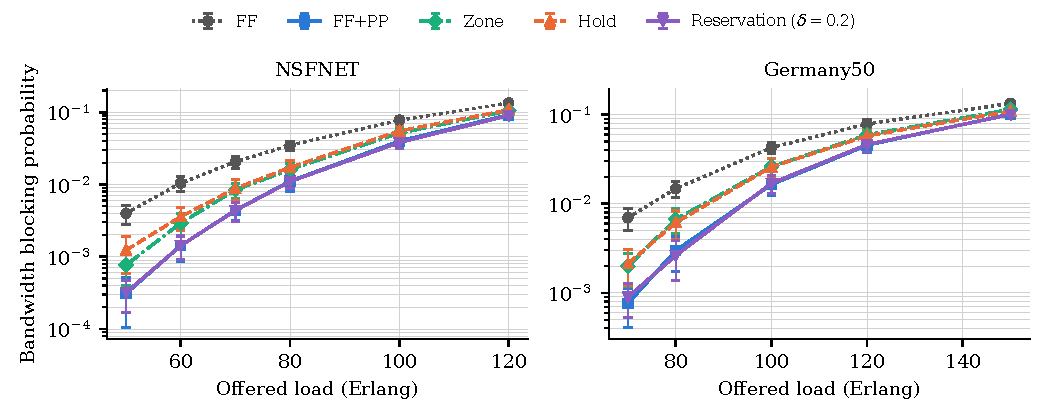
\includegraphics[width=\textwidth]{j_fig_bbp.pdf}
\caption{Bandwidth blocking probability versus offered load on NSFNET and Germany50 ($\phi=0.3$, 10 seeds, 95\% confidence intervals).}
\label{fig:bbp}
\end{figure}

Fig.~\ref{fig:rounds} shows the cost of this gain. The number of shifts per run grows from about 2{,}500 to 78{,}000 between 50 and 120 Erlang on NSFNET, and from 5{,}400 to 79{,}000 between 70 and 150 Erlang on Germany50. Grouping the shifts into rounds of routes that share no link reduces the number of sequential steps by a factor of 2.5--3.3 on NSFNET and 3.3--3.7 on Germany50. The factor is larger on Germany50 because its many links give more routes that do not overlap, and it grows with load because each Push-Pull pass moves more lightpaths. Defragmentation therefore finishes three to four times faster at the same final spectrum state.

\begin{figure}[t]
\centering
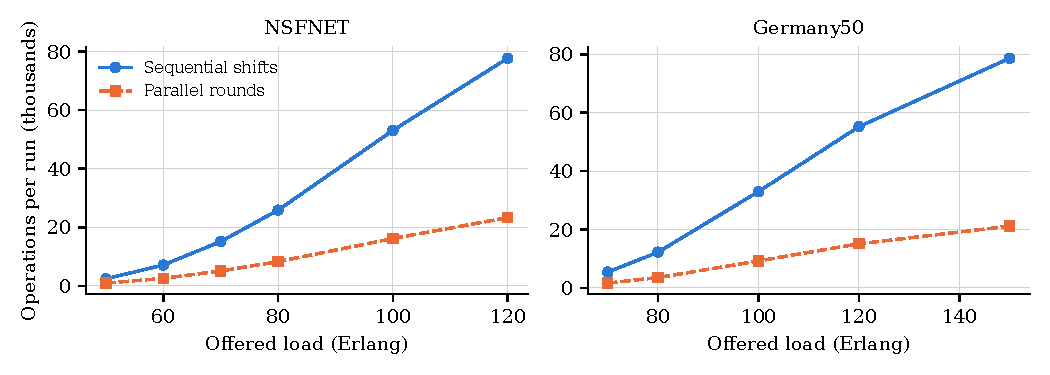
\includegraphics[width=\textwidth]{j_fig_rounds.pdf}
\caption{Push-Pull operations per run with FF+PP: sequential shifts versus parallel rounds after route grouping.}
\label{fig:rounds}
\end{figure}

\subsection{Detection accuracy}
Without timing jitter, the detector is almost exact. On NSFNET, reservations have a precision of 1.00, i.e., every reservation is used by the expected request, and a recall of 0.92 at 80 Erlang, falling to 0.86 at 120 Erlang. On Germany50 the precision is also 1.00 and the recall falls from 0.99 at 70 Erlang to 0.91 at 150 Erlang. The missing recall is not caused by wrong detections but by reservations that fail for lack of free spectrum at high load. Hold has a precision of 0.98--0.99 on both topologies; the few unused held blocks belong to flows whose next repeat is blocked or detected late.

\subsection{Pattern-based schemes at a fixed lead}
Tables~\ref{tab:nsf} and~\ref{tab:g50} compare the schemes. With the default lead $\delta=0.2$, Reservation does not change BBP significantly at any load on either topology. It lowers the blocking of periodic requests by a small amount, 11--13\% at 100--150 Erlang, which is significant in the paired test. The reason for the small effect is that the block is reserved only shortly before the request arrives: when a block is free at that moment, the request would usually have found one anyway.

Hold lowers the blocking of periodic requests by 25--36\% at 80--120 Erlang on NSFNET and by 25--41\% at 100--150 Erlang on Germany50, because their spectrum is not released between repeats. The held blocks, however, stay idle until the next repeat. Random requests are therefore blocked 41--85\% more often on NSFNET and 33--98\% more often on Germany50 at the same loads, and total BBP rises significantly at every load. At low load, Hold does not help periodic flows at all, since they are rarely blocked, and only adds cost.

Zone reduces the number of Push-Pull shifts by 42--60\% on NSFNET at 80--120 Erlang and by 26--61\% on Germany50 at 80--150 Erlang, because the two classes no longer interleave. It raises BBP significantly at every load, by 14--45\% on NSFNET at 80--120 Erlang and by 13--160\% on Germany50, because each class can use only part of the band efficiently. Zone+Hold adds the costs of both.

\input{tables_fmt}

\subsection{Tuning the trade-off}\label{sec:tradeoff}
The results so far suggest that the useful question is not whether pattern knowledge lowers total blocking, but how cheaply it can protect periodic traffic. Fig.~\ref{fig:tradeoff} places each scheme by the blocking it causes to random requests (horizontal axis) and to periodic requests (vertical axis) at 100 Erlang. Points further down and to the left are better.

\begin{figure}[t]
\centering
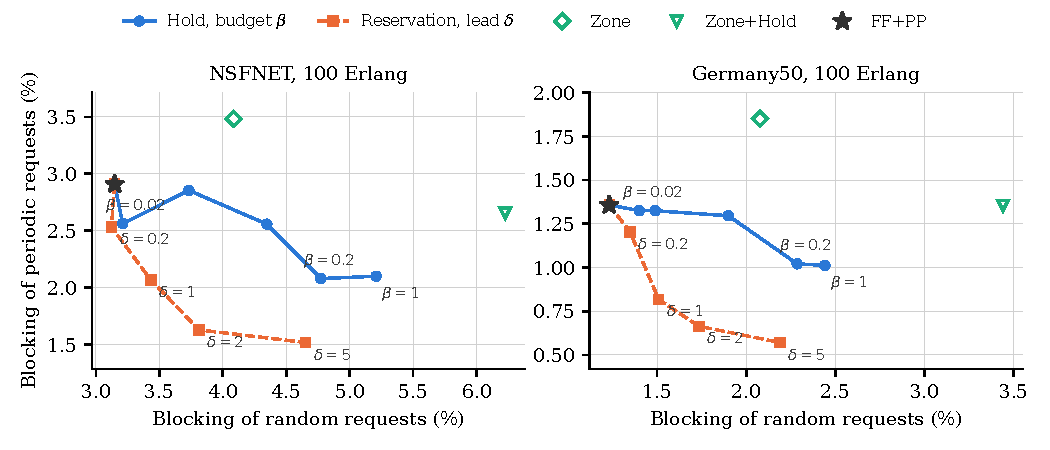
\includegraphics[width=\textwidth]{j_fig_tradeoff.pdf}
\caption{Blocking of periodic versus random requests at 100 Erlang (mean of 10 seeds). Curves start at FF+PP and vary the reservation lead $\delta$ and the Hold budget $\beta$ ($\beta=1$ is unrestricted Hold).}
\label{fig:tradeoff}
\end{figure}

\paragraph{Reservation lead} Lengthening the lead moves Reservation along a much better curve than Hold on both topologies. On NSFNET, $\delta=1$ (about 7.5\% of the period) lowers the blocking of periodic requests by 29\% with no significant change in BBP ($-2\%$), and $\delta=2$ lowers it by 44\% with no significant change in BBP ($+3\%$), although random blocking rises by 21\%. Only at $\delta=5$ does the idle reserved spectrum raise BBP significantly ($+21\%$). On Germany50, $\delta=1$ lowers periodic blocking by 40\% with no significant change in BBP ($+3\%$), at $+23\%$ random blocking; $\delta=2$ gives $-51\%$ at a small but significant BBP increase ($+11\%$). Unrestricted Hold gives less protection ($-28\%$ and $-25\%$) at a much higher cost ($+38\%$ and $+58\%$ BBP), because a held block stays idle for the whole gap between repeats instead of a short lead.

This holds across loads. On NSFNET, Reservation with $\delta=1$ lowers periodic blocking significantly, by 29--49\% at 60--120 Erlang, without a significant change in BBP at any load from 50 to 120 Erlang (Table~\ref{tab:nsf}).

\paragraph{Hold budget} On NSFNET, a small budget makes Hold cheaper: at $\beta=0.02$, periodic blocking falls by 12\% at 100 Erlang and 9\% at 120 Erlang with no significant change in BBP, and larger budgets move toward unrestricted Hold. The curve is not monotone ($\beta=0.05$ at 100 Erlang), which reflects the noise of 10 seeds. On Germany50, budgets up to $\beta=0.1$ give no significant protection while still raising random blocking. A budget of $\beta S\approx 6$ slots admits only the smallest blocks, and on Germany50 a held block occupies more links, so it reaches the budget sooner. The budget is therefore a weaker and less portable knob than the reservation lead.

\subsection{Effect of the share of periodic traffic}\label{sec:phi}
Fig.~\ref{fig:phi} varies the share $\phi$ of periodic load on NSFNET at 100 Erlang, with the reservation lead scaled to 7.5\% of the period in each case. Reservation and Hold give similar protection to periodic flows: 42--48\% at $\phi\le0.2$, falling to 16--19\% at $\phi\ge0.4$. The relative protection falls as $\phi$ grows because the protected class becomes a larger part of the traffic, so it competes more with itself. The cost differs sharply. Reservation leaves BBP unchanged at every $\phi$ (paired change between $-3\%$ and $+4\%$, none significant), whereas Hold raises BBP by 25--48\%.

\begin{figure}[t]
\centering
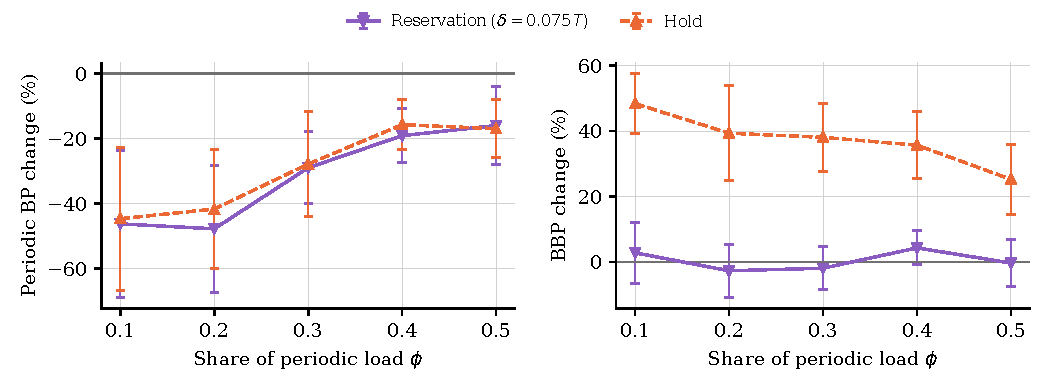
\includegraphics[width=\textwidth]{j_fig_phi.pdf}
\caption{Effect of the share of periodic load $\phi$ on NSFNET at 100 Erlang: paired change relative to FF+PP in the blocking of periodic requests (left) and in BBP (right), with 95\% paired confidence intervals.}
\label{fig:phi}
\end{figure}

\subsection{Robustness to timing jitter}\label{sec:jitter}
Real scheduled services do not start exactly on time. Fig.~\ref{fig:jitter} shows Hold on NSFNET at 100 Erlang when each periodic arrival is shifted by Gaussian noise with standard deviation $\sigma$. With $\varepsilon=0.1$, recall falls from 0.91 to 0.65 at $\sigma=0.05$ and to 0.24 at $\sigma=0.1$, and the protection of periodic flows disappears: their blocking returns to the FF+PP level. With $\varepsilon=0.3$, recall stays above 0.9 up to $\sigma=0.05$ and is 0.82 at $\sigma=0.1$, while precision stays between 0.89 and 0.98. A tolerance of about three standard deviations of the jitter is therefore needed. In practice, $\varepsilon$ can be set from the observed spread of the inter-arrival times of each key.

\begin{figure}[t]
\centering
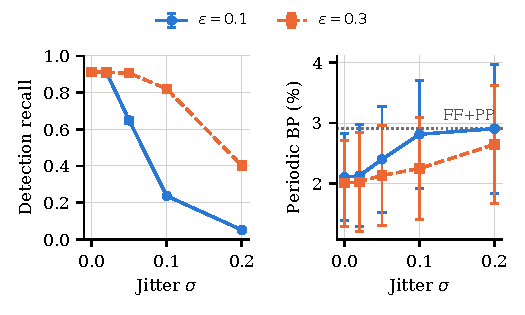
\includegraphics[width=0.6\textwidth]{fig_jitter.pdf}
\caption{Hold under arrival-time jitter $\sigma$ on NSFNET at 100 Erlang for two detection tolerances $\varepsilon$: detection recall (left) and blocking of periodic requests (right, 95\% confidence intervals).}
\label{fig:jitter}
\end{figure}

\subsection{Predictability of per-pair demand}
Table~\ref{tab:dt} shows the decision-tree results. When 30--50\% of the load comes from periodic flows, the tree predicts high-demand windows with a precision of 0.91--0.97 but a recall of only 0.27--0.37, because only the pairs that carry periodic flows are predictable. With little or no periodic traffic, the F1-score is near zero. On the OPNET trace used in \cite{malayeri2022}, the precision of 0.54 equals the share of positive windows, i.e., chance level. Re-examining that trace showed why: its offered load is about 5{,}000 Erlang, and the generator wrote the periodic requests to a separate file, so the trace contains no recurring pattern to learn. This explains the small gain reported in the thesis.

\begin{table}[t]
\centering
\caption{Decision-tree prediction of high-demand windows (mean of 10 seeds for synthetic traffic).}
\label{tab:dt}
\small
\begin{tabular}{@{}lrrr@{}}
\toprule
Traffic & Precision & Recall & F1 \\
\midrule
Synthetic, $\phi=0$ & 0.43 & 0.00 & 0.01 \\
Synthetic, $\phi=0.1$ & 0.52 & 0.02 & 0.03 \\
Synthetic, $\phi=0.3$ & 0.91 & 0.27 & 0.42 \\
Synthetic, $\phi=0.5$ & 0.97 & 0.37 & 0.54 \\
OPNET trace of \cite{malayeri2022} & 0.54 & 0.97 & 0.69 \\
\bottomrule
\end{tabular}
\end{table}

% ===============================================================
\section{Discussion}\label{sec:discussion}
% ===============================================================
The results answer the three questions of the introduction.

\paragraph{Where the gains come from} The large and reliable reductions in blocking come from defragmentation itself (24--92\% lower BBP than First-Fit), and running it in parallel rounds makes it three to four times faster. Pattern knowledge adds nothing to total blocking: under the same offered load, every use of it that we tested either leaves BBP unchanged or raises it.

\paragraph{Detection} Periodic flows can be detected from the request stream with simple rules, no training and constant work per request, with a precision close to 1. The detector is sensitive to timing jitter, but a tolerance of about three standard deviations of the jitter restores a recall above 0.8.

\paragraph{How to use the patterns} Knowing which requests will come lets the network decide \emph{who} receives the spectrum. This is useful for service differentiation, for example to protect scheduled video services during busy hours. The price of this protection is the time the spectrum is kept idle. Hold keeps it idle for the whole gap between repeats and is therefore expensive. Reservation keeps it idle only for the lead time and, with a lead of about one tenth of the period, lowers the blocking of periodic flows by 29--49\% on NSFNET and 40\% on Germany50 without a significant change in total blocking. Zone is not a protection mechanism at all; it is a way to halve defragmentation work at the cost of blocking, which may be acceptable when re-tuning is slow or risky.

\paragraph{Practical use} The schemes need no change to the data plane. Detection and reservation run in the controller, for example in a software-defined network controller that already sees every request. The reservation lead and the detection tolerance are the two parameters to set; the first fixes the trade-off between periodic and random traffic, and the second should follow the measured jitter of the scheduled services.

\paragraph{Limitations} The study uses a single modulation format, uniform node pairs and synthetic periodic flows with Gaussian jitter. Real traffic may contain daily patterns, flows whose period or bandwidth drifts, and flows that recur at irregular times. With distance-adaptive modulation, the bandwidth of a flow would depend on its path, which the detector would need to take into account. Finally, results on measured traffic traces would be the strongest test of the conclusions. The simulator is open, so all of these cases can be added.

% ===============================================================
\section{Conclusion}\label{sec:conclusion}
% ===============================================================
We studied whether recognizing recurring traffic patterns reduces the blocking caused by spectrum fragmentation in elastic optical networks. On NSFNET and Germany50, grouped Push-Pull defragmentation lowered blocking by 24--92\% compared with First-Fit and ran three to four times faster thanks to independent-set route grouping. Periodic flows were detected with a precision of 1.00 and a recall of 0.86--0.99, but no use of them lowered total blocking. Holding spectrum protected periodic flows by up to 41\% and a separate zone cut defragmentation shifts by up to 61\%, each at a clear cost to other traffic. Reserving spectrum about one tenth of a period ahead gave 29--49\% protection without a significant change in total blocking, on both topologies and for periodic shares from 10\% to 50\%, and a detection tolerance of three times the timing jitter kept the recall above 0.8. Pattern awareness therefore does not create capacity; it decides which traffic receives it, and advance reservation with a short lead is the cheapest way to do so. Future work includes distance-adaptive modulation, measured traffic, priority classes for scheduled services, and learning when pattern-based actions pay off.

\section*{CRediT authorship contribution statement}
\textbf{Mohammad Mahdi Malayeri:} Conceptualization, Methodology, Software, Investigation, Formal analysis, Visualization, Writing -- original draft. \textbf{Mohsen Nickray:} Conceptualization, Supervision, Writing -- review \& editing. \todo{Confirm roles with Dr Nickray.}

\section*{Declaration of competing interest}
The authors declare that they have no known competing financial interests or personal relationships that could have appeared to influence the work reported in this paper.

\section*{Data availability}
The simulator, all experiment scripts and the raw results are openly available at \url{https://github.com/malayerimahdi/EON-Pattern-Aware-Spectrum-Management}.

\section*{Declaration of generative AI and AI-assisted technologies in the writing process}
\todo{Elsevier requires a statement if AI tools were used to prepare the manuscript, code or figures. Complete this according to the journal's policy, e.g.: ``During the preparation of this work the authors used Claude (Anthropic) to help write simulation code and edit the text. After using this tool, the authors reviewed and edited the content as needed and take full responsibility for the content of the publication.''}


\bibliographystyle{elsarticle-num}
\begin{thebibliography}{99}

\bibitem{jinno2009}
M. Jinno \textit{et al.}, ``Spectrum-efficient and scalable elastic optical path network: Architecture, benefits, and enabling technologies,'' \textit{IEEE Commun. Mag.}, vol.~47, no.~11, pp.~66--73, 2009.

\bibitem{gerstel2012}
O. Gerstel, M. Jinno, A. Lord, and S. J. B. Yoo, ``Elastic optical networking: A new dawn for the optical layer?,'' \textit{IEEE Commun. Mag.}, vol.~50, no.~2, pp.~s12--s20, 2012.

\bibitem{chatterjee2015}
B. C. Chatterjee, N. Sarma, and E. Oki, ``Routing and spectrum allocation in elastic optical networks: A tutorial,'' \textit{IEEE Commun. Surveys Tuts.}, vol.~17, no.~3, pp.~1776--1800, 2015.

\bibitem{abkenar2017}
F. S. Abkenar and A. G. Rahbar, ``Study and analysis of routing and spectrum allocation (RSA) and routing, modulation and spectrum allocation (RMSA) algorithms in elastic optical networks (EONs),'' \textit{Opt. Switch. Netw.}, vol.~23, pp.~5--39, 2017.

\bibitem{shen2015}
J. Shen, J. Chen, and Y. Sun, ``Fragmentation aware routing and spectrum assignment algorithm for elastic optical networks,'' in \textit{Proc. IEEE TENCON}, 2015.

\bibitem{athari2019}
A. Athari Beyragh, A. G. Rahbar, S.-M. Hosseini Ghazvini, and M. Nickray, ``IF-RSCA: Intelligent fragmentation-aware method for routing, spectrum and core assignment in space division multiplexing elastic optical networks (SDM-EON),'' \textit{Opt. Fiber Technol.}, vol.~50, pp.~284--301, 2019.

\bibitem{patel2011}
A. N. Patel, P. N. Ji, J. P. Jue, and T. Wang, ``Defragmentation of transparent flexible optical WDM (FWDM) networks,'' in \textit{Proc. OFC/NFOEC}, 2011.

\bibitem{wang2013}
R. Wang and B. Mukherjee, ``Provisioning in elastic optical networks with non-disruptive defragmentation,'' \textit{J. Lightw. Technol.}, vol.~31, no.~15, 2013, doi: 10.1109/JLT.2013.2268535.

\bibitem{zhang2013}
M. Zhang, W. Shi, L. Gong, W. Lu, and Z. Zhu, ``Bandwidth defragmentation in dynamic elastic optical networks with minimum traffic disruptions,'' in \textit{Proc. IEEE ICC}, 2013.

\bibitem{cugini2013}
F. Cugini \textit{et al.}, ``Push-pull defragmentation without traffic disruption in flexible grid optical networks,'' \textit{J. Lightw. Technol.}, vol.~31, no.~1, pp.~125--133, 2013.

\bibitem{shakya2013}
S. Shakya and X. Cao, ``Spectral defragmentation in elastic optical path networks using independent sets,'' in \textit{Proc. OFC/NFOEC}, 2013.

\bibitem{lu2013ar}
W. Lu and Z. Zhu, ``Dynamic service provisioning of advance reservation requests in elastic optical networks,'' \textit{J. Lightw. Technol.}, vol.~31, no.~10, pp.~1621--1627, 2013.

\bibitem{chino2016}
M. Chino, T. Miyazaki, E. Oki, S. Okamoto, and N. Yamanaka, ``Adaptive elastic spectrum allocation based on traffic fluctuation estimate in flexible OFDM-based optical networks,'' in \textit{Proc. IEEE HPSR}, 2016.

\bibitem{panayiotou2019}
T. Panayiotou, K. Manousakis, S. P. Chatzis, and G. Ellinas, ``A data-driven bandwidth allocation framework with QoS considerations for EONs,'' \textit{J. Lightw. Technol.}, vol.~37, no.~9, pp.~1853--1864, 2019.

\bibitem{salani2019}
M. Salani, C. Rottondi, and M. Tornatore, ``Routing and spectrum assignment integrating machine-learning-based QoT estimation in elastic optical networks,'' in \textit{Proc. IEEE INFOCOM}, 2019, pp.~1738--1746.

\bibitem{malayeri2022}
M. M. Malayeri, ``Optimization of fragmented spectrum in elastic optical networks using pattern recognition,'' M.Sc. thesis, Dept. Comput. Eng. IT, Univ. of Qom, Qom, Iran, 2022 (in Persian).

\bibitem{talebi2014}
S. Talebi, F. Alam, I. Katib, M. Khamis, R. Salama, and G. N. Rouskas, ``Spectrum management techniques for elastic optical networks: A survey,'' \textit{Opt. Switch. Netw.}, vol.~13, pp.~34--48, 2014.

\bibitem{yen1971}
J. Y. Yen, ``Finding the $k$ shortest loopless paths in a network,'' \textit{Manage. Sci.}, vol.~17, no.~11, pp.~712--716, 1971.

\bibitem{chen2019}
X. Chen, B. Li, R. Proietti, H. Lu, Z. Zhu, and S. J. B. Yoo, ``DeepRMSA: A deep reinforcement learning framework for routing, modulation and spectrum assignment in elastic optical networks,'' \textit{J. Lightw. Technol.}, vol.~37, no.~16, pp.~4155--4163, 2019.

\bibitem{orlowski2010}
S. Orlowski, R. Wess\"aly, M. Pi\'oro, and A. Tomaszewski, ``SNDlib 1.0---Survivable network design library,'' \textit{Networks}, vol.~55, no.~3, pp.~276--286, 2010.

\bibitem{natalino2020}
C. Natalino and P. Monti, ``The Optical RL-Gym: An open-source toolkit for applying reinforcement learning in optical networks,'' in \textit{Proc. Int. Conf. Transparent Optical Networks (ICTON)}, 2020, doi: 10.1109/ICTON51198.2020.9203239.

\bibitem{trindade2021}
S. Trindade, R. da S. Torres, Z. Zhu, and N. L. S. da Fonseca, ``Cognitive control-loop for elastic optical networks with space-division multiplexing,'' \textit{Sensors}, vol.~21, no.~23, art.~7821, 2021.

\bibitem{etezadi2022}
E. Etezadi, C. Natalino, R. Diaz, A. Lindgren, S. Melin, L. Wosinska, P. Monti, and M. Furdek, ``DeepDefrag: A deep reinforcement learning framework for spectrum defragmentation,'' in \textit{Proc. IEEE GLOBECOM}, 2022, pp.~3694--3699.

\bibitem{etezadi2023}
E. Etezadi, C. Natalino, R. Diaz, A. Lindgren, S. Melin, L. Wosinska, P. Monti, and M. Furdek, ``Deep reinforcement learning for proactive spectrum defragmentation in elastic optical networks,'' \textit{J. Opt. Commun. Netw.}, vol.~15, no.~10, pp.~E86--E96, 2023.

\bibitem{davalos2023}
E. D\'avalos, J.-L. Enciso, N. Silva, J. Pinto-R\'ios, and A. Leiva, ``Triggering strategy for defragmentation process in elastic optical networks using machine learning techniques,'' \textit{ICT Express}, vol.~9, no.~5, pp.~890--895, 2023.

\end{thebibliography}
\end{document}
